\section{Quantum Fourier Transformation}
We have already encountered the quantum phase estimation \textsc{qpe} where we assumed to have access to the quantum Fourier transformation \textsc{qft}. In the following we will see how to realize it.\\

\subsection{Discrete Fourier Transformation} 
\begin{def*}[\texttt{DFT}]
The classical discrete Fourier transformation \textsc{dft} on $N$ complex numbers $\left
\{ x_k
\right\}_{k=0}^{D-1}$ generated as new set of complex numbers $\left
\{ X_k
\right\}_{k=0}^{D-1}$ given by
\begin{align}
    X_k = \frac{1}{\sqrt{D}} \sum_{l=0}^{D-1} x_l e^{2\pi i \frac{kl}{D}}.
\end{align}
\end{def*}
We can write the initial numbers $x_l$ as vector and the Fourier transform as matrix $U_{\textsc{FT}}$ 
\begin{align}
    \mathbf{X} = U_{\textsc{FT}} \mathbf{x}
\end{align} 
with matrix elements
\begin{align}
    (U_{\textsc{FT}})_{kl} = \frac{1}{\sqrt{D}} e^{2\pi i \frac{kl}{D}}.
\end{align}
This matrix is unitary
\begin{align}
    \left(U_{\textsc{FT}}^\dagger U_{\textsc{FT}}\right)_{kl} &= \sum_{m} \left(U_{\textsc{FT}}^\dagger\right)_{km} \left(U_{\textsc{FT}}\right)_{ml}\\
    &=\sum_{m} \left(U_{\textsc{FT}}\right)_{mk}^* \left(U_{\textsc{FT}}\right)_{ml}\\
    &=\frac{1}{D}\sum_{m} e^{-2\pi i \frac{mk}{D}} e^{2\pi i \frac{ml}{D}}\\
    &=\frac{1}{D}\sum_{m} e^{2\pi i\frac{m}{D}\left(l - k\right)}\\
    &=\delta_{kl}.
\end{align}
For $k=l$ this is fairly easy to see
\begin{align}
    \frac{1}{D}\sum_{m} e^{0 } = \frac{1}{D} D = 1,
\end{align}
for $k\neq l$ we first need to remember that the sum over all $D$th unit-roots (the numbers $e^{2\pi \frac{k}{D}}$ with $k=0,1,\dots D-1$) is zero
\begin{align}
    \sum_{m<D} e^{2\pi i\frac{m}{D}} = 0.
\end{align}
and the same if we change the direction
\begin{align}
    \sum_{m<D} e^{-2\pi i\frac{m}{D}} = 0.
\end{align}
To see this: draw them on the complex unit circle and verify that for each vector representing the complex unit roots there is another one that corresponds to the same vector in opposite direction. All that is left now, is to realize that $e^{i2\pi p \alpha} = e^{i2\pi \alpha} $ and $e^{-i2\pi p \alpha} = e^{-i2\pi \alpha} $ for any positive integer $p$. So no matter if positive or negative, since we have $l-k = \pm p$ the sum $\sum_{m<D} e^{2\pi i (l-k) \frac{m}{D}}$  will always vanish.

\subsection{Quantum Fourier Transformation}
The quantum Fourier transform \textsc{qft} on $N$ qubits can now be realized with the same unitary matrix as the discrete Fourier transform with dimension $D=2^N$. Instead of $D$ complex numbers it will act on the $D = 2^N$ binary basis states of the $N$-qubits.
\begin{def*}[\texttt{QFT}]
The quantum fourier transform takes the standard basis states $\ket{k}$ on $N$ qubits and transforms them into
\begin{align}
    \ket{\hat{k}} = \textsc{qft} \ket{k} = \frac{1}{\sqrt{2^N}}\sum_{l<2^N} e^{2\pi i \frac{kl}{2^N}}\ket{l}.\label{eq:qft}
\end{align}
\end{def*}
It may come as a surprise, but the transformed state $\ket{\hat{k}}$ is actually a product state -- so we are changing from the non-entangled standard basis $\ket{k}$ to the non-entangled Fourier basis $\ket{\hat{k}}$. Lets go step by step.
\subsubsection*{1-Qubit}
\begin{algo*}[\texttt{QFT}(N=1)]
 For a single qubit the \textsc{QFT} is the same as the \textsc{Hadamard} transformation
\begin{align}
    \textsc{QFT} = \frac{1}{\sqrt{2}} \begin{pmatrix}
        1 & 1 \\ 1 & -1 
    \end{pmatrix} = \textsc{H}.
\end{align}   
\end{algo*}

The transformed states are
\begin{align}
    \ket{0} \rightarrow \ket{\hat{0}}&=\ket{+}\\
    \ket{1} \rightarrow \ket{\hat{1}}&=\ket{-}.
\end{align}
Admitedly, that was not very exciting.
\subsubsection*{2-Qubits}
The now 4-dimensional \textsc{QFT} is
\begin{align}
    \textsc{QFT} = \frac{1}{2} \begin{pmatrix}
        1 & 1 & 1 & 1 \\
        1 & e^{2\pi \frac{1\cdot 1}{4}} & e^{2\pi \frac{1\cdot 2}{4}} & e^{2\pi \frac{1\cdot 3}{4}} \\
        1 & e^{2\pi \frac{2\cdot 1}{4}} & e^{2\pi \frac{2\cdot 2}{4}} & e^{2\pi \frac{2\cdot 3}{4}} \\
        1 & e^{2\pi \frac{3\cdot 1}{4}} & e^{2\pi \frac{3\cdot 2}{4}} & e^{2\pi \frac{3\cdot 3}{4}} \\
    \end{pmatrix} = \frac{1}{2} \begin{pmatrix}
        1 & 1 & 1 & 1 \\
        1 & i & -1 & -i \\
1 & -1 & 1 & -1 \\
1 & -i & -1 & i \\
    \end{pmatrix}
\end{align}
leading to the following basis states
\begin{align}
    \ket{00}   &\rightarrow  \frac{1}{2}\left( \ket{00} + \ket{01} + \ket{10} + \ket{11} \right) = \ket{+}\otimes\ket{+}\\
    \ket{01}   &\rightarrow  \frac{1}{2}\left( \ket{00} + i\ket{01} - \ket{10} -i \ket{11} \right) = \ket{-}\otimes\ket{+i}\\
    \ket{10}   &\rightarrow  \frac{1}{2}\left( \ket{00} - \ket{01} +\ket{10} -\ket{11} \right) = \ket{+}\otimes\ket{-}\\
    \ket{11}   &\rightarrow  \frac{1}{2}\left( \ket{00} -i \ket{01} - \ket{10} +i \ket{11} \right) = \ket{-}\otimes\ket{-i}\\
\end{align}
with the usual $\ket{\pm}$ states and the ``Y-States''\footnote{$\ket{\pm}$ are eigenstates of Pauli-X while $\ket{\pm i}$ are eigenstates of Pauli-Y}
\begin{align}
    \ket{\pm i} = \frac{1}{\sqrt{2}}\left(\ket{0} \pm i \ket{1} \right).
\end{align}
We can construct the $\ket{\pm i}$ from the $\ket{\pm}$ by introducing a ``phase gate'' 
\begin{align}
    R(\varphi) = \begin{pmatrix}
        1 & 0 \\ 0 & e^{i\varphi}
    \end{pmatrix}
\end{align}
and then have
\begin{align}
    \ket{\pm i} = R(\pi/2) \ket{\pm}.
\end{align}
We can start with just two Hadamard gates, which gives us the mapping:
\begin{align}
    \ket{00} &\xrightarrow{\mathsc{H}\otimes \mathsc{H}} \ket{++} \\
    \ket{01} &\xrightarrow{\mathsc{H}\otimes \mathsc{H}} \ket{+-} \\
    \ket{10} &\xrightarrow{\mathsc{H}\otimes \mathsc{H}} \ket{-+} \\
    \ket{11} &\xrightarrow{\mathsc{H}\otimes \mathsc{H}} \ket{--} \\
\end{align}
which is a bit disappointing in the end, as it only gets the $\ket{00} \rightarrow \ket{++}$ correct. Through further inspection we see however, that the mapping of $\ket{10}$ is almost correct, just the wrong order -- we can however fix this with a \textsc{SWAP} gate.
\vspace{0.25cm}
\noindent\rule{\textwidth}{0.4pt}
\vspace{0.25cm}
The SWAP gate swaps two basis states $\textsc{SWAP}\ket{i}\otimes\ket{j} = \ket{j}\otimes\ket{i}$ and by linearity it swaps general product states $\textsc{SWAP}\ket{\phi}\otimes\ket{\psi} = \ket{\psi}\otimes\ket{\phi}$. We can realize it with 3 \textsc{cnot} gates (try it for yourself).
\vspace{0.25cm}
\noindent\rule{\textwidth}{0.4pt}
\vspace{0.25cm}
Now we are almost there:
\begin{align}
    \ket{00} &\xrightarrow{\textsc{SWAP}\left(\mathsc{H}\otimes \mathsc{H}\right)} \ket{++} \\
    \ket{01} &\xrightarrow{\textsc{SWAP}\left(\mathsc{H}\otimes \mathsc{H}\right)} \ket{-+} \\
    \ket{10} &\xrightarrow{\textsc{SWAP}\left(\mathsc{H}\otimes \mathsc{H}\right)} \ket{+-} \\
    \ket{11} &\xrightarrow{\textsc{SWAP}\left(\mathsc{H}\otimes \mathsc{H}\right)} \ket{--} \\
\end{align}
the only thing left is to change the states on the right qubit in the $\ket{01}\rightarrow \ket{-+}$ mapping from $\ket{+}$ to $\ket{+i}$ and similar in the $\ket{11}\rightarrow \ket{--}$ mapping from $\ket{-}$ to $\ket{-i}$. We can do this by applying the $R$ operation given above to the right qubit after the \textsc{SWAP} operation, or to the left qubit before the \textsc{SWAP} operation. No matter the choice we will however introduce $\ket{+i}$ and $\ket{-i}$ states in the mapping of $\ket{00}$ and $\ket{10}$. In order to avoid this we perform a controlled-$R$ operation where we take the left qubit as a control bit -- now we \textit{have} to do it \textit{before} the \textsc{SWAP} operation. The final Fourier transform for 2 qubit is then given by
\begin{align}
    \ket{00} &\xrightarrow{\textsc{SWAP}\;\left(1\otimes \mathsc{H}\right)\;CR\;\left(\mathsc{H}\otimes 1\right)} \ket{+}\otimes\ket{+} \\
    \ket{01} &\xrightarrow{\textsc{SWAP}\;\left(1\otimes \mathsc{H}\right)\;CR\;\left(\mathsc{H}\otimes 1\right)} \ket{-}\otimes\ket{+i} \\
    \ket{10} &\xrightarrow{\textsc{SWAP}\;\left(1\otimes \mathsc{H}\right)\;CR\;\left(\mathsc{H}\otimes 1\right)} \ket{+}\otimes\ket{-} \\
    \ket{11} &\xrightarrow{\textsc{SWAP}\;\left(1\otimes \mathsc{H}\right)\;CR\;\left(\mathsc{H}\otimes 1\right)} \ket{-}\otimes\ket{-i} \\
\end{align}
with the control-qubit in $CR$ being the right qubit. We can represent this as a quantum circuit using the upper wire as the left qubit and the lower wire as the right qubit
\begin{align}
    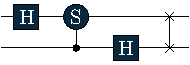
\includegraphics[width=0.4\textwidth]{src/circuit_qft_2qubits.pdf}
\end{align}
Note, that the operation $R(\pi/2)$ is often denoted as $S$ which is common for this special angle
\begin{align}
   R(\pi/2) = \begin{pmatrix}
        1 & 0 \\ 0 & i 
    \end{pmatrix} \equiv S
\end{align}

\subsubsection*{3-Qubits}
Same game as before. We have the Matrix
\begin{align}
\frac{1}{\sqrt{8}}
    \begin{pmatrix}
1 & 1 & 1 & 1 & 1 & 1 & 1 & 1 \\
1 & e^{2\pi i \frac{1}{8}} & e^{2\pi i \frac{2}{8}} & e^{2\pi i \frac{3}{8}} & e^{2\pi i \frac{4}{8}} & e^{2\pi i \frac{5}{8}} & e^{2\pi i \frac{6}{8}} & e^{2\pi i \frac{7}{8}} \\
1 & e^{2\pi i \frac{2}{8}} & e^{2\pi i \frac{4}{8}} & e^{2\pi i \frac{6}{8}} & e^{2\pi i \frac{8}{8}} & e^{2\pi i \frac{10}{8}} & e^{2\pi i \frac{12}{8}} & e^{2\pi i \frac{14}{8}} \\
1 & e^{2\pi i \frac{3}{8}} & e^{2\pi i \frac{6}{8}} & e^{2\pi i \frac{9}{8}} & e^{2\pi i \frac{12}{8}} & e^{2\pi i \frac{15}{8}} & e^{2\pi i \frac{18}{8}} & e^{2\pi i \frac{21}{8}} \\
1 & e^{2\pi i \frac{4}{8}} & e^{2\pi i \frac{8}{8}} & e^{2\pi i \frac{12}{8}} & e^{2\pi i \frac{16}{8}} & e^{2\pi i \frac{20}{8}} & e^{2\pi i \frac{24}{8}} & e^{2\pi i \frac{28}{8}} \\
1 & e^{2\pi i \frac{5}{8}} & e^{2\pi i \frac{10}{8}} & e^{2\pi i \frac{15}{8}} & e^{2\pi i \frac{20}{8}} & e^{2\pi i \frac{25}{8}} & e^{2\pi i \frac{30}{8}} & e^{2\pi i \frac{35}{8}} \\
1 & e^{2\pi i \frac{6}{8}} & e^{2\pi i \frac{12}{8}} & e^{2\pi i \frac{18}{8}} & e^{2\pi i \frac{24}{8}} & e^{2\pi i \frac{30}{8}} & e^{2\pi i \frac{36}{8}} & e^{2\pi i \frac{42}{8}} \\
1 & e^{2\pi i \frac{7}{8}} & e^{2\pi i \frac{14}{8}} & e^{2\pi i \frac{21}{8}} & e^{2\pi i \frac{28}{8}} & e^{2\pi i \frac{35}{8}} & e^{2\pi i \frac{42}{8}} & e^{2\pi i \frac{49}{8}} \\
    \end{pmatrix}
\end{align}
A common notation that makes things easier is to use the abbreviation $\omega = e^{2\pi i \frac{1}{8}} $ and realize that $\omega^8 = \omega^0 = 1$ and $\omega^9 = \omega^1$ (because $e^{2\pi i}=1$) and $\omega^4 = -1$ etc, which gives
\begin{align}
\frac{1}{\sqrt{8}}
\begin{pmatrix}
1 & 1 & 1 & 1 & 1 & 1 & 1 & 1 \\
1 & \omega^1 & \omega^2 & \omega^3 & -1 & \omega^5 & \omega^6& \omega^7 \\
1 & \omega^2 & -1 & \omega^6 & 1 & \omega^2 & -1 &\omega^6 \\
1 & \omega^3 & \omega^6 & \omega^1 & -1 & \omega^7 & \omega^2& \omega^5 \\
1 & -1 & 1 & -1 & 1 & -1 & 1 & -1 \\
1 & \omega^5 & \omega^2 & \omega^7 & -1 & \omega^1 & \omega^6& \omega^3 \\
1 & \omega^6 & -1 & \omega^2 & 1 & \omega^6 & -1 &\omega^2 \\
1 & \omega^7 & \omega^6 & \omega^5 & -1 & \omega^3 & \omega^2 & \omega^1 \\
 \end{pmatrix}.
\end{align}
We can again get the first and middle transformation correct by using a sequence of Hadamard operations followed by swapping the qubit order
\begin{align}
    \ket{000} &\rightarrow \ket{+++}\\ 
    \ket{100} &\rightarrow \ket{++-}.
\end{align}
Let's look at the transformation of the second basis state
\begin{align}
    \ket{001} &\rightarrow \frac{1}{\sqrt{8}} \left( \ket{000} + \omega^1\ket{001} + \omega^2\ket{010} + \omega^3\ket{011} - \ket{100} + \omega^5 \ket{101} + \omega^6 \ket{110} + \omega^7 \ket{111} \right)\nonumber
\end{align}
note that $\omega^2 = i$ and $\omega^6 = -i$ (so $\omega^2 = - \omega^6$) and also $\omega^5 = -\omega^1$ as well as $\omega^7 = - \omega^3$ (draw them on the complex unit circle to see it for yourself), so we have
\begin{align}
    \ket{001} &\rightarrow \frac{1}{\sqrt{8}} \left( \ket{000} + \omega^1\ket{001} + \omega^2\ket{010} + \omega^3\ket{011} - \ket{100} - \omega^1 \ket{101} - \omega^2 \ket{110} - \omega^3 \ket{111} \right)\nonumber
\end{align}
which we can further simplify to
\begin{align}
 \ket{-} \otimes \frac{1}{2}\left(\ket{00} + \omega^1\ket{01} + \omega^2\ket{10} + \omega^3\ket{11}\right).
\end{align}
Further simplification comes by realizing that $\omega^3 = \omega^1\cdot \omega^2$, so that we end up with
\begin{align}
 \ket{-} \otimes \frac{1}{\sqrt{2}}\left(\ket{0} + \omega^2 \ket{1}\right)\otimes \frac{1}{\sqrt{2}}\left(\ket{0} + \omega^1 \ket{1}\right),
\end{align}
so we are ending up with a product state again, the three individual states can be created with a Hadamard and the $R(\theta)$ operation tuned to the correct angle -- in this case we have the angles $R(\theta=\pi/4) = S$ (as before) and $R(\theta=\pi/8) = T$. To ensure that we are not messing with the $\ket{000}\rightarrow\ket{+++}$ and $\ket{100}\rightarrow\ket{++-}$ transformation we will control the two operations with the rightmost qubit and afterwards swap the qubit order again, the circuit that performs this operation is
\begin{align}
    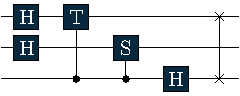
\includegraphics[height=0.1\textheight]{src/circuit_qft_3qubits_pre.pdf}.
\end{align}
With this we are almost there, there are just a few states left that are not yet transformed correctly. One of them is the last basis state should transform as
\begin{align}
    \ket{111} &\rightarrow \frac{1}{4} \left( \ket{000} + \omega^7\ket{001} + \omega^6\ket{010} + \omega^5\ket{011} - \ket{100} + \omega^3 \ket{101} + \omega^2 \ket{110} + \omega^1 \ket{111} \right)\nonumber\\
\end{align}
using our identities from before
\begin{align}
    \ket{111} &\rightarrow \frac{1}{4} \left( \ket{000} + \omega^7\ket{001} + \omega^6\ket{010} + \omega^5\ket{011} - \ket{100} - \omega^7 \ket{101} - \omega^4 \ket{110} - \omega^7 \ket{111} \right)\nonumber\\
    &= \ket{-} \otimes \frac{1}{2}\left( \ket{00} + \omega^7\ket{01} + \omega^6\ket{10} + \omega^5\ket{11}\right).
\end{align}
Now, remember the periodicity again and realize that $\omega^7 \cdot \omega^6 = \omega^{13} = \omega^5$
\begin{align}
    \ket{111} &\rightarrow \ket{-}\otimes \frac{1}{\sqrt{2}}\left(\ket{0} + \omega^6\ket{1}\right)\otimes\frac{1}{\sqrt{2}}\left(\ket{0} + \omega^7\ket{1}\right)
\end{align}
or, in our case more convenient
\begin{align}
    \ket{111} &\rightarrow \ket{-}\otimes \frac{1}{\sqrt{2}}\left(\ket{0} - \omega^2\ket{1}\right)\otimes\frac{1}{\sqrt{2}}\left(\ket{0} - \omega^3\ket{1}\right).
\end{align}
This is almost the same state as we already had above for the $\ket{001}$ transformation, except for the minus signs (they will however be correctly introduced by the Hadamard transformations, now acting on qubits in $\ket{1}$ and not $\ket{0}$) and the frequency in the rightmost qubit which is $\omega^3$ instead of $\omega^1$. To get the correct frequency we can modify the circuit with an additional controlled-$S$ operation (note that $S$ acting on $\omega^1\ket{1}$ will lead to $\omega^2\omega^1\ket{1 = \omega^3\ket{1}}$). We place the control on the central qubit (so the operation will be switched off in the $\ket{001}$ transformation above). 
The final circuit for the 3-Qubit \textsc{QFT} is then
\begin{align}
    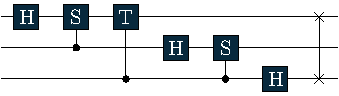
\includegraphics[height=0.1\textheight]{src/circuit_qft_3qubits.pdf},
\end{align}
this circuit transforms all states correctly -- verification on the remaining 4 states is left as an exercise.

\subsection*{N-Qubits}
\begin{algo*}[\texttt{QFT}]\phantom{...}\\
The circuit for the quantum Fourier transform on $N$ qubits can be assembled
\begin{algorithmic}
\STATE $\textsc{qft} = \left[\right] $
\FOR{$ 1 \leq n \leq N$}
\STATE $ \texttt{qft} += \hd(n) \texttt{qft} $
\FOR{$1\leq m \leq  N-n$}
\STATE $ \texttt{qft} += CR\left(n+m,n,\frac{\pi}{2^{m+1}}\right)$
\ENDFOR
\ENDFOR
\FOR{$1 \leq n \leq $ $ \lfloor{N/2}\rfloor$}
\STATE $\texttt{qft} += \texttt{SWAP}(n,N-(n-1))$
\ENDFOR
\RETURN $\texttt{qft}$
\end{algorithmic}
Here we used "$+=$" to indicate the assembling of gates in a list. 
\end{algo*}
